\chapter{Realisierung Objekterkennung}\label{kap:object_det}

In diesem Kapitel werden zunächst die Beschaffung und Aufbereitung 
der Trainingsdaten beschrieben. Anschließend wird es um das 
Training geeigneter Deep-Learning-Modelle in \textit{TensorFlow}
 sowie um die \Gls{inferenz} dieser Modelle in \textit{OpenVino} gehen.

\section{Datensatz}\label{sec:dataset}

Für das Training eines Deep-Learning-Modells werden 
eine Große Menge an Trainingsdaten benötigt.
Handelt es sich um ein Modell zur Objekterkennung
müssen die Labels neben der Klasse auch die Koordinaten 
der Bounding-Boxen enthalten.

Die Trainingsdaten können entweder selber erstellt oder 
aus frei zugänglichen Datensätzen wie z.B. \textit{ImageNet}, 
\textit{COCO}, oder \textit{Open Images}
aus dem Internet heruntergeladen werden.

Für die Bachelorarbeit wurden aus dem Open Source Datensatz
\textit{Open Images} von Google
\cite{kuznetsovaOpenImagesDataset2018}, 
welches 600 gelabelte Klassen enthält, 
die 9 Klassen \textit{Brown bear, Deer, Fox, Goat, 
Hedgehog, Owl, Rabbit, Raccoon} und \textit{Squirrel}
heruntergeladen und für das Training verwendet.

Für die Evaluierung des Trainings wurde der 
Datensatz, in ein
Trainings-, ein Validierungs- und ein 
Testset aufgeteilt, mit einem Verhältnis von 80\%, 10\%, 10\%.

Bei den verschiedenen Klassen variierte die Anzahl der 
Bilder zwischen 200 und 
2000 Stück, wodurch eine Verteilung der Klassen, 
wie in dem in Abbildung \ref{fig:histo_ohne_aug} dargestelltem
Histogramm, zustandekam.

\vspace{1cm}
\begin{minipage}{0.5\textwidth}
    \centering
    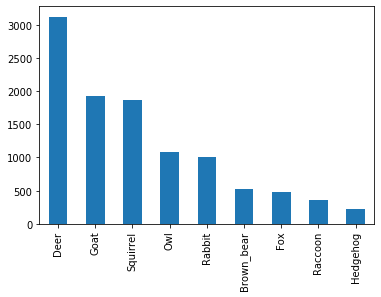
\includegraphics[width=0.9\textwidth]{class_distro.png}
    \captionof{figure}{Verteilung der Klassen}
    \label{fig:histo_ohne_aug}
\end{minipage}
\begin{minipage}{0.5\textwidth}
    \centering
    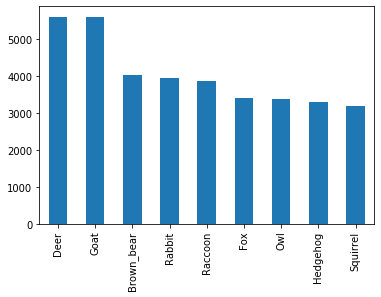
\includegraphics[width=0.9\textwidth]{class_distro_aug.png}
    \captionof{figure}{Verteilung der Klassen
     nach Augmentierung der Daten}
    \label{fig:histo_mit_aug}
\end{minipage}
\vspace{1cm}

Um diese quantitativen Unterschiede auszugleichen,
wurden die Daten, wie im nächsten
Abschnitt genauer beschrieben wird, so augmentiert, 
dass für jede Klasse 3000 Bilder vorhanden waren,
was zu einer in Abbildung \ref{fig:histo_mit_aug} 
dargestellten Verteilung führte.

Da sich häufig mehrere Tiere derselben Klasse 
auf einem Bild befinden, weicht, wie in den Histogrammen 
zu erkennen ist, die Anzahl der Bilddateien (3000) von 
der Anzahl der Klassen ab.



\subsection{Augmentierung}\label{subsec:augmentation}

Das Augmentieren von Bilddaten für Deep-Learning-Modelle
erfolgt, indem geometrische Transformationen oder Manipulationen 
an den Pixelwerten auf die Bilder angewendet werden.
Die Anzahl der Bilder wird durch dieses Verfahren 
künstlich vermehrt.
Neben dem Ausgleich der Klasseninbalance ist dies 
auch eine sehr effektive Technik, um
Overfitting zu verhindern.

Die Augmentierung des \textit{Open Images} Datensatzes 
wurde mithilfe eines Python-Scripts, in welchem die Library 
\textit{imgaug} \cite{imgaug} verwendet wurde, durchgeführt.
Dabei wurde, für jedes zu augmentierendem Bild eine geometrische und 
eine pixelbezogene Transformation angewendet, die 
zufällig aus einer Auswahl an Augmentern ausgewählt wurde.

In folgendem Codeausschnitt des Python-Scripts sind die 
verwendeten Augmentierungstechniken dargestellt:

\begin{lstlisting}[language=Python]
    import imgaug.augmenters as iaa
    
    color_augmenters = [
        iaa.Dropout(p=(0, 0.1)),
        iaa.CoarseDropout((0.01, 0.05), size_percent=0.1),
        iaa.Multiply((0.5, 1.3), per_channel=(0.2)),
        iaa.GaussianBlur(sigma=(0, 5)),
        iaa.AdditiveGaussianNoise(scale=((0, 0.2*255))),
        iaa.ContrastNormalization((0.5, 1.5)),
        iaa.Grayscale(alpha=((0.1, 1))),
        iaa.ElasticTransformation(alpha=(0, 5.0), sigma=0.25),
        iaa.PerspectiveTransform(scale=(0.15)),
        iaa.MultiplyHueAndSaturation((0.7))
    ]

    geometric_augmenters = [
        iaa.Affine(scale=((0.6, 1.2))),
        iaa.Affine(translate_percent=(-0.3, 0.3)),
        iaa.Affine(shear=(-25, 25)),
        iaa.Affine(translate_percent={"x": (-0.3, 0.3), "y": (-0.2, 0.2)}),
        iaa.Fliplr(1),
        iaa.Affine(scale={"x": (0.6, 1.4), "y": (0.6, 1.4)})
    ]
    
\end{lstlisting}

Das Ergebnis von einigen zufällig angewendeten Augmentierungen 
auf ein Bild der Klasse Fuchs ist
in Abbildung \ref{fig:augmentierung} dargestellt:

\begin{figure}[H]
    \centering
    \includegraphics[width=0.95\columnwidth]{Bilder/augmentierung.png}
    \caption{Beispielhafte Augmentierungsergebnisse 
    für Bilder der Klasse \textit{Fuchs}}
    \label{fig:augmentierung}
\end{figure}


\section{Object detection Modelle}

Object detection Modelle lassen sich
in einstufige- und zweistufige Detektoren einteilen,
siehe \cite{wuRecentAdvancesDeep2019} für eine 
Ausführliche Beschreibung

Zweistufige Detektoren generieren in der 
ersten Stufe eine Auswahl an räumlichen Vorschlägen
für das Inputbild, in dem Objekte enthalten sein 
können. 
In der zweiten Stufe werden die Vorschläge zur \textit{Feature 
Extraction} einem \Gls{cnn} übergeben, welches neben 
einem \textit{Klassifikator} auch einen \textit{Regressor} für 
die Bounding-Box-Koordinaten besitzt.

Einstufige Verfahren verwenden kein separates 
Netz zur Vorschlagsgenerierung. Stattdessen 
wird das gesamte Bild als potentielle
Region für Objekte betrachtet, indem 
dieses gitterartig unterteilt wird.
Jeder Teil, der eine mögliche Region darstellt, 
wird dann hinsichtlich des Vorhandensein 
eines Objekts klassifiziert.

Für diese Bachelorarbeit wurden 
Modelle beider Ansätze verwendet und 
hinsichtlich Genauigkeit und 
\Gls{inferenz}zeit miteinander verglichen.
Im Folgenden werden die beiden 
verwendeten Modelle näher erläutert.


\subsection*{Faster R-CNN}

Das Faster R-CNN \cite{renFasterRCNNRealTime2016a} 
ist ein Modell zur Objekterkennung, welches
ein zweistufiges Verfahren verwendet und 
in Abbildung \ref{fig:faster_rcnn} 
dargestellt ist.
Die Vorschlagsgenerierung erfolgt in einem 
\textit{\Gls{rpn}}, welches auf 
einem \textit{fully convolutional network} 
basiert.
Über die generierten \textit{\Glspl{featuremap}} werden im 
\textit{Sliding-Window}-Verfahren vordefinierte
\textit{Anker Boxen} konvoliert.
Der daraus resultierende Feature-Vektor wird 
einem binären Klassifikator (\textit{cls layer}), 
der angibt ob, sich ein Objekt
in dem Vorschlag befindet, 
sowie einem Bounding-Box-Regresor
(\textit{reg layer}) zur Lokalisierung,
übergeben.

\vspace{1cm}
\begin{figure}[H]
    \centering
    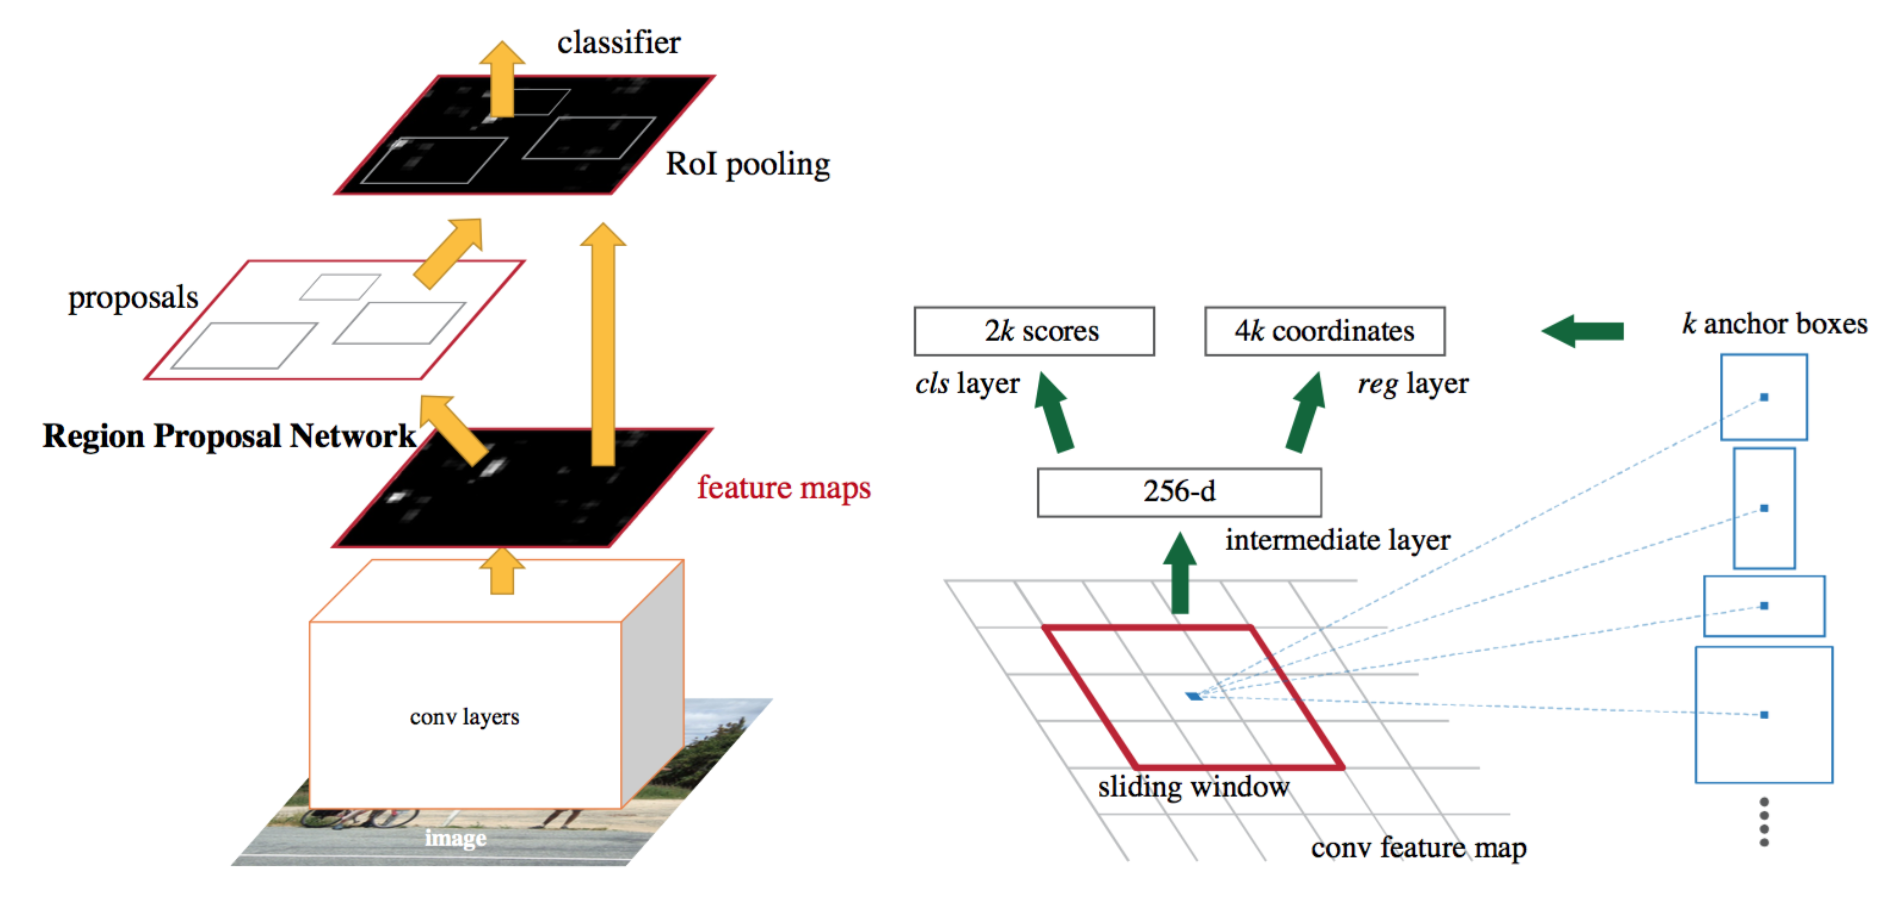
\includegraphics[width=0.95\textwidth]
    {faster-RCNN_architecture.png}
    \caption{Faster R-CNN Architektur
     \cite{renFasterRCNNRealTime2016a}}
     \label{fig:faster_rcnn}
\end{figure}

\subsection*{SSD: Single Shot MultiBox Detector}

Der Single Shot MultiBox Detector (SSD)
 \cite{liuSSDSingleShot2016}
verwendet ein einstufiges Verfahren zur Objekterkennung,
bei dem das Inputbild gitterartig unterteilt wird.
In jeder Zelle des Gitters werden \textit{default Anker
Boxen} unterschiedlicher Skalierungen definiert.

Indem an das Basis-\Gls{cnn} weitere \textit{Extra Feature Layer}
verschiedener Größen angehängt werden, kann dieses 
für jede default-Box eine Klassifikation in Form 
eines \textit{confidence scores}, sowie eine Lokalisierung 
in Form eines \textit{Offsets} zur default-Box, vornehmen.

Diese werden zur finalen Detektion 
einem \textit{non-maximum suppression}
Layer übergeben, der Boxen, die der selben Klasse angehören 
zusammenführt.\cite{hosangLearningNonmaximumSuppression2017}


\begin{figure}[H]
    \centering
    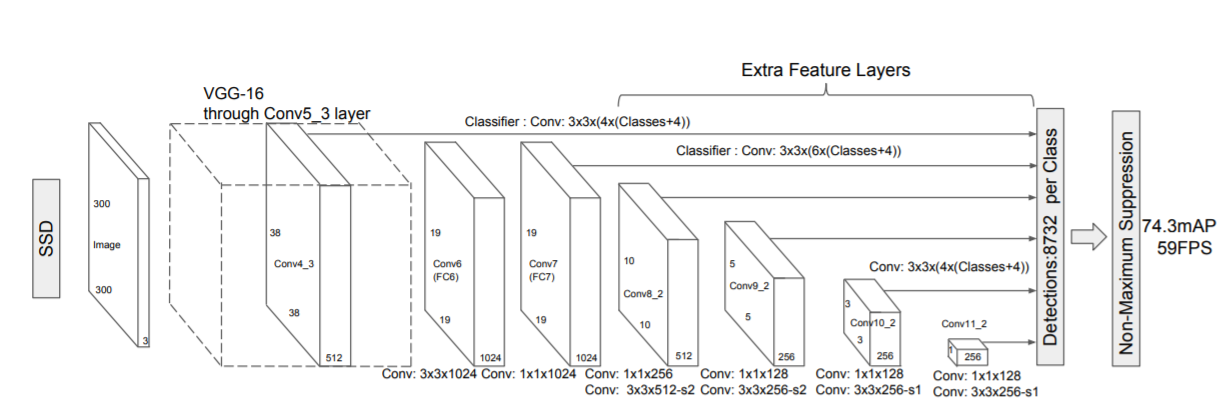
\includegraphics[width=0.95\textwidth]
    {ssd_architecture.png}
    \caption{SSD Architektur \cite{liuSSDSingleShot2016}}
    \label{fig:faster_rcnn}
\end{figure}



\section{Training}

Das Training der Deep-Learning-Modelle erfolgte in dem 
\Gls{framework} \textit{TensorFlow}, welches auch von 
\textit{OpenVino} für den \textit{Neural Compute Stick}
unterstützt wird.
Dabei wurde eine speziell für die Objekterkennung 
entwickelte \Gls{api} von \textit{TensorFlow} verwendet.

Um unabhängig von der Leistungsfähigkeit der \Gls{gpu} des 
Rechners zu sein wurde das Training in der Cloudbasierten
\Gls{vm} \textit{Google Colab} \cite{colab} durchgeführt,
die eine für Deep Learning geeignete,
\Gls{gpu} kostenlos zur Verfügung stellt.



\subsection{TensorFlow Object Detection API}

Die \textit{TensorFlow Object Detection API} ist unter den
Research Modellen des offiziellen TensorFlow
Repositorys auf \textit{GitHub} zu finden \cite{tfobjdet}
und enthält Implementierungen
einiger gängiger Object-detection-Modelle mit verschiedenen 
vortrainerten Basis-\Glspl{cnn}.

Der für diese Bachelorarbeit verwendete Single 
Shot Detector (SSD) wurde zum einen mit dem 
MobilenetV2 und zum anderen mit dem 
InceptionV2 als Basis CNN trainiert.
Für das Faster R-CNN wurde aufgrund 
der Verfügbarkeit nur mit dem InceptionV2
trainiert.

Um die Modelle trainieren zu können, mussten zunächst die 
Trainingsdaten in das von der TensorFlow \Gls{api}
verwendete binäre Dateiformat \textit{TFRecords} 
umgewandelt werden.
Dieses ist eine serialisierte Darstellung der Bilder
 und Labelfiles als \textit{Protocol Buffer},
welche einen schnellen Zugriff auf die Daten ermöglichen.

Parameter für das Modell konnten vor dem Training 
in einer Konfigurationsdatei festgelegt werden.
Diese wurde dann zusammen mit den \textit{TFRecord}-Dateien 
dem Konsolen-Kommando mit dem das Training 
gestartet wurde, übergeben.

Während des Trainings wurden in regelmäßigen 
Abständen die trainierten Gewichte abgespeichert.

Mithilfe des Evaluierungstools \textit{TensorBoard}
konnte der Trainingsfortschritt anhand bestimmter
Metriken angezeigt und ausgewertet werden. So konnten schon während des Trainings fehlerhafte
Einstellungen der Datensatz- und 
Modellkonfiguration festgestellt 
und korrigiert werde, indem z.B. andere
Augmentierungstechniken verwendet
oder \textit{Hyperparameter} des
Modells umgestellt wurden.

In Abbildung \ref{fig:train_workflow}
ist der so entstandene Trainingsworkflow dargestellt.

Die Ergebnisse der trainierten Modelle 
werden im nächsten Kapitel diskutiert.
\vspace{1cm}

\begin{figure}[H]
    \centering
    
\tikzstyle{process} = [rectangle, fill=blue!20, node distance=4cm, minimum width=1.5cm, minimum height=0.8cm, text centered, draw=black]
\tikzstyle{arrow} = [thick,->,>=stealth]
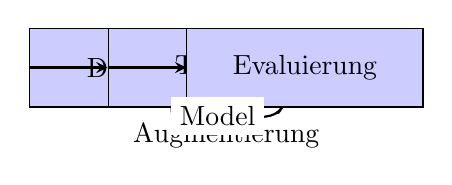
\begin{tikzpicture}[scale=0.4]
      \node (data)      [process]                   {Datensatz};
      \node (train)      [process, right of=data]      {Training};
      \node (eval)      [process, right of=train]      {Evaluierung};
    \draw[arrow] (data) -- (train);
    \draw[arrow] (train) -- (eval);
  \draw[arrow] (eval) edge[bend left=60] node [centered, fill=white!30] {Augmentierung} (data);
  \draw[arrow] (eval) edge[bend left=60] node [left, fill=white!30] {Model} (train);
\end{tikzpicture}

% \begin{tikzpicture}[scale=0.4]

%   \begin{scope}[node distance=3cm]

%    \node (data)      [process]                   {Datensatz};
%    \node (prep)      [process, right of=data]      {Aufbereitung};
%    \node (model)      [process, right of=prep]      {Model};
%    \node (train)      [process, right of=model]      {Training};
%    \node (eval)      [process, right of=train]      {Evaluierung};

%   \end{scope}

%  \draw[arrow] (data) -- (prep);
%  \draw[arrow] (prep) -- (model);
%  \draw[arrow] (model) -- (train);
%  \draw[arrow] (train) -- (eval);
 

% \draw[arrow] (eval) edge[bend left=60] node [left, fill=white!30] {ändern} (data);
% \draw[arrow] (eval) edge[bend left=60] node [left, fill=white!30] {augment} (prep);
% \draw[arrow] (eval) edge[bend left=60] node [left, fill=white!30] {ändern} (model);
% \draw[arrow] (eval) edge[bend left=60] node [left, fill=white!30] {Parameter} (train);

 
% \end{tikzpicture}

    \caption{Trainingsworkflow}
    \label{fig:train_workflow}
\end{figure}
\vspace{1cm}


\section{\Gls{inferenz}}\label{sec:inferenz}

Zur Ausführung der \Gls{inferenz} eines fertig trainierten 
Modells auf dem \textit{Neural Compute Stick 2} 
wird das Toolkit \textit{OpenVino} von \textit{Intel} verwendet.
Dafür musste zunächst der trainierte \textit{TensorFlow Graph} 
exportiert, d.h. die aktuellen Werte der Gewichte 
eingefroren werden.
Anschließend konnte mit dem \textit{Model Optimizer}
das Modell in die \textit{Intermediate Representation} (IR)
konvertiert werden.
Diese besteht aus einer .xml- und einer .bin-Datei und 
und kann von der \textit{Inference Engine}
zur \Gls{inferenz} gelesen werden.


\subsection*{Inference Engine}

Um die \Gls{inferenz} eines Modells im IR-Format 
auf dem NCS2 ausführen zu können werden 
in der \textit{Inference Engine} die in Abbildung 
\ref{fig:inger_engine_workflow} schematisch
dargestellten Schritte durchgeführt.
Daneben ist jeweils die entsprechende 
Codezeile in Python angegeben.

Zunächst wird das Zielgerät, auf dem 
die \Gls{inferenz} ausgeführt werden soll,
spezifiziert (\textit{HW Plugin laden}).
Anschließend wird das Modell anhand der 
IR-Dateien definiert (\textit{Model IR einlesen})
woraus sich die \textit{In}- und \textit{Outputblobs}
 generieren lassen (\textit{In-und Outputblob}), 
Diese stellen die Dimensionen der Ein- und Ausgabeschicht
des Modells darstellen.
Das zu inferierende Bild,
dass als Matrix aus Pixelwerten 
vorliegt, muss dann in das \textit{Input Blob}
Format gebracht werden (\textit{process Input}).
Nachdem das Bild inferiert wurde (\textit{\Gls{inferenz}}),
kann es zusammen mit den \Gls{inferenz}ergebnissen 
weiterverarbeitet werden (\textit{process
output}).
Handelt es sich bei den Inputs 
um einen fortlaufenden Video- oder 
Kamerastream, werden die Schritte 
\textit{preprocess}, \textit{\Gls{inferenz}} und 
\textit{process Output} in einer Schleife wiederholt.


\vspace{1cm}
\begin{minipage}{0.30\textwidth}
    \centering
    
\tikzstyle{process} = [rectangle, fill=blue!20, minimum width=3cm, minimum height=1cm, text centered, draw=black]
\tikzstyle{arrow} = [thick,->,>=stealth]

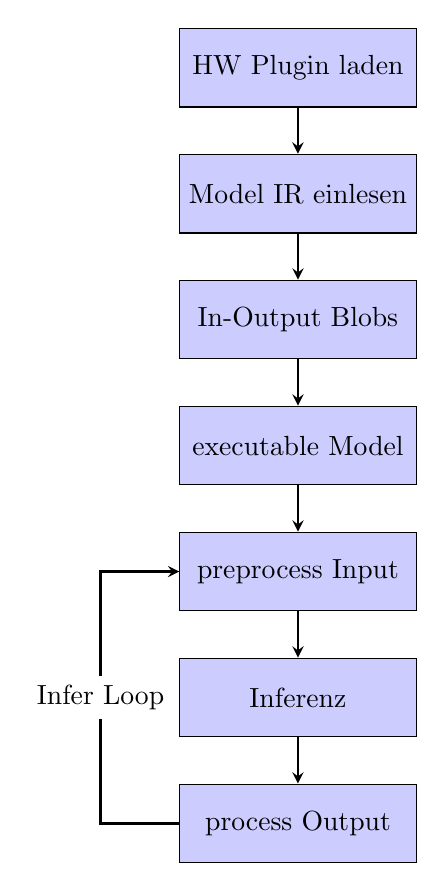
\begin{tikzpicture}[node distance=1.6cm]
    \node (hw)      [process]                   {HW Plugin laden};
    \node (ir)      [process, below of=hw]      {Model IR einlesen};
    \node (io)      [process, below of=ir]      {In-Output Blobs};
    \node (execNet) [process, below of=io]      {executable Model};
    \node (prepIn)  [process, below of=execNet] {preprocess Input};
    \node (infer)   [process, below of=prepIn]  {Inferenz};
    \node (procOut) [process, below of=infer]   {process Output};

    \draw [arrow] (hw) -- (ir);
    \draw [arrow] (ir) -- (io);
    \draw [arrow] (io) -- (execNet);
    \draw [arrow] (execNet) -- (prepIn);
    \draw [arrow] (prepIn) -- (infer);
    \draw [arrow] (infer) --  (procOut);

    \draw [arrow] (procOut.west) -- +(-1,0) |- node[pos=0.25, fill=white!30] {Infer Loop} (prepIn);

    
\end{tikzpicture}

    \captionof{figure}{Programmab-lauf der
    InferenceEngine}
    \label{fig:inger_engine_workflow}
\end{minipage}
\begin{minipage}{0.70\textwidth}

%\begin{python}
\begin{lstlisting}[language=Python]

    plugin = IEPlugin(device='MYRIAD')

        
    net = IENetwork(model_xml, model_bin)
        
    
    input_blob  = net.inputs
    output_blob = net.outputs
        

    exec_net = plugin.load_network(net, n_req)
        
    while True:

        image = preprocess(capture) # hwc -> nchw
        
        
        res = exec_net.infer({input_blob : image})
        

        res = res[output_blob]
        
        
\end{lstlisting}
%\end{python}
\vspace{1.5cm}
\end{minipage}
\vspace{1cm}

% transform:
% # capture dims zu input blob dims transformieren
% # img_h, img_w, img_c -> blob_n, blob_c, blob_h, blob_w

Die Form des \Gls{inferenz}ergebnisses hängt von der 
Art des verwendeten Deep-Learning-Modells ab, z.B.
\textit{Image Classification}, \textit{Object detection},
oder \textit{Instance
Segmentation}.

Für Object-detection-Modelle enthält das Ergebnis
 Datenstrukturen, die den Index, 
 die zugehörige Wahrscheinlichkeit sowie die 
 Bounding-Box-Koordinaten der geschätzen Objekte im Bild enthalten.

Indem für alle Schätzungen, die in einem Bild gemacht wurden, 
ein Threshold für die Wahrscheinlichkeit festlegt wird (zb. bei 70\%),
können die sinnvollen Ergebnisse herausgefiltert werden.

Zur Veranschaulichung können die Koordinaten dann 
als Bounding-Box in das inferierte Bild gezeichnet werden.
